\documentclass{article}
\usepackage{amsmath}
\usepackage{hyperref}
\usepackage{graphicx}
\usepackage{adjustbox}
\newcommand{\tabincell}[2]{\begin{tabular}{@{}#1@{}}#2\end{tabular}}

\begin{document} %This is where document begins
\begin{titlepage}
\title{EE 232E \\Graphs and Network Flows\\Homework 1\\Winter 2016} 
\author{Liqiang Yu, Rongjing Bai, Yunwen Zhu\\
904592975, 504592374, 304588434}  %change your ID here
\date{04-12-2016}
\end{titlepage}

\maketitle
\newpage
\tableofcontents
\newpage

\section{Problem1}\label{prob:p1}
This is problem \ref{prob:p1} shown with reference.
\subsection{Part a}
\subsection{Part b}

\section{Problem2}
Table \ref{tb:simple} is a simple table.\\
\\
Table \ref{tb:complex} is a complex table.
\begin {table}[htbp]
\caption{A simple table}
\begin{adjustbox}{center}
\label{tb:simple}
\begin{tabular}{|c|c|c|}
\hline
1&2&3\\
\hline
4&5&6\\
\hline
\end{tabular}
\end{adjustbox}
\end{table}


\begin{table}[hbp]
\caption{The data information for each hashtag}
\begin{adjustbox}{center}
\label{tb:complex}
\begin{tabular}{|c|c|c|c|c|c|c|}
\hline
& gohawks & gopatriots & nfl &patriots & sb49 & superbowl\\
\hline
\tabincell{c}{Average number of \\tweets per hour} & 380.84 & 53.43 & 515.98 & 975.52 & 1647.31 & 2692.14\\
\hline
\tabincell{c}{Average number of \\follower per users}& 1544.97 & 1298.82 & 4289.75 & 1650.32 & 2235.16 & 3591.60\\
\hline
\tabincell{c}{Average number of \\retweets per tweet}& 2.01& 1.40 & 1.54 & 1.78 & 2.51 & 2.39\\
\hline
\end{tabular}
\end{adjustbox}
\end{table}

\section{Problem 3}
Figure \ref{fig:sp_hist} shows how to insert a figure, "htbp" means the position preference, here top bottom and whatever p is (sorry I forgot).
\begin{figure}[htbp]
\centering
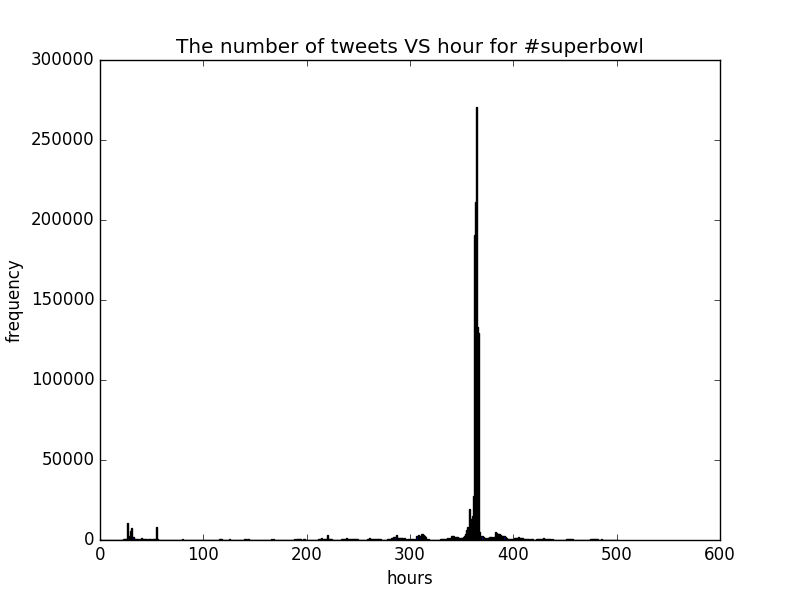
\includegraphics[width=.6\textwidth]{sp_hist.png}
\caption{The histogram for \#SuperBowl}
\label{fig:sp_hist}
\end{figure}

\section{Problem 4}
\subsection{Formula}
Here is how to insert a seperate formula.\\
\begin{equation*}
PMI(t_1, t_2) = log\left( \frac{P(t_1\cap t_2)}{P(t_1)*P(t_2)}\right) 
\end{equation*} 
\\
And here is a multi-lines formula.\\
\begin{equation*}
\begin{split}
&P(t) =\frac{DF(t)}{|D|}\\
&P(t_1\cap t_2) = \frac{DF(t1\cap t2)}{|D|}
\end{split}
\end{equation*}
\\
If you want to use inline formula, you can use \$ to wrap around it, like hi this is an inline formula example $P(t) =\frac{DF(t)}{|D|}$ which is pretty easy right.
\subsection{Some other things}
Please do use the \large{\textbf{reference}} to label all the figures and tables, with the command label and ref.\\
\\
Please pay attention to how to start a new paragraph, usually with two set of double-slash, like the following paragraphs.\\
\\
We choose to use \#gohawks and \#patriots as the support hashtag for two teams because the amount of data in \#gopatriots is too small. We split the data into one hour period and only consider the 24 hours around the game. We plot the semantic orientation every hour for the twitter contents from two teams fans and make the comparison. \\
\\
The results are shown in figure. From the figure we can see that at first seahawks fans are more confident than patriots fans, however there was a turning point at around  6:30pm, which is 3 hour after the game start. When we enlarge that area and show it in figure, we can see that after that turning point patriots fans are much happier than hawks fans. After referring it to the game facts, we think it makes sense because it describes a story of bouncing back from behind and win the championship. \\
\\
The table shows the game facts. From the game facts, we can see that at 190 minutes, which is nearly 3 hours after the game start, the hawks lead the patriots by 24:14, however after that the hawks got no point anymore and the patriots turned back and won the superbowl. Therefore it explained why hawks fans started to feel unhappy at the time 3 hours after the game start and why patriots felt happy.

\end{document}
